% \part{Template}\label{part:template}
\chapter{Towards atom-photon entanglement}\label{ch:atomphoton}

% the hierarchy is 
% chapter,section,subsection,etc.

\section{Single photon generation}
A precursor to preparing Bell state between single atoms and emitted photons is the ability to generate a photon from an atom on-demand. With an atom optically pumped into $\ket{5S_{1/2},F=1,m_F=0}$ as described in the previous chapter, $\pi$-polarized 780 nm light incident on the atom can excite it to $\ket{5P_{3/2},F=1,m_F=0}$, where the spontaneous decay is expected to be in a single photon Fock state. Unlike some remote entanglement protocols which involve weak excitation\cite{cabrillo1999creation}, with an intentionally small probability of exciting the atom, here we employ a $\pi$ pulse so that the population is entirely in the excited state to maximize the per-excitation chance of extracting a photon. 

\begin{figure}[!h]
    \centering
    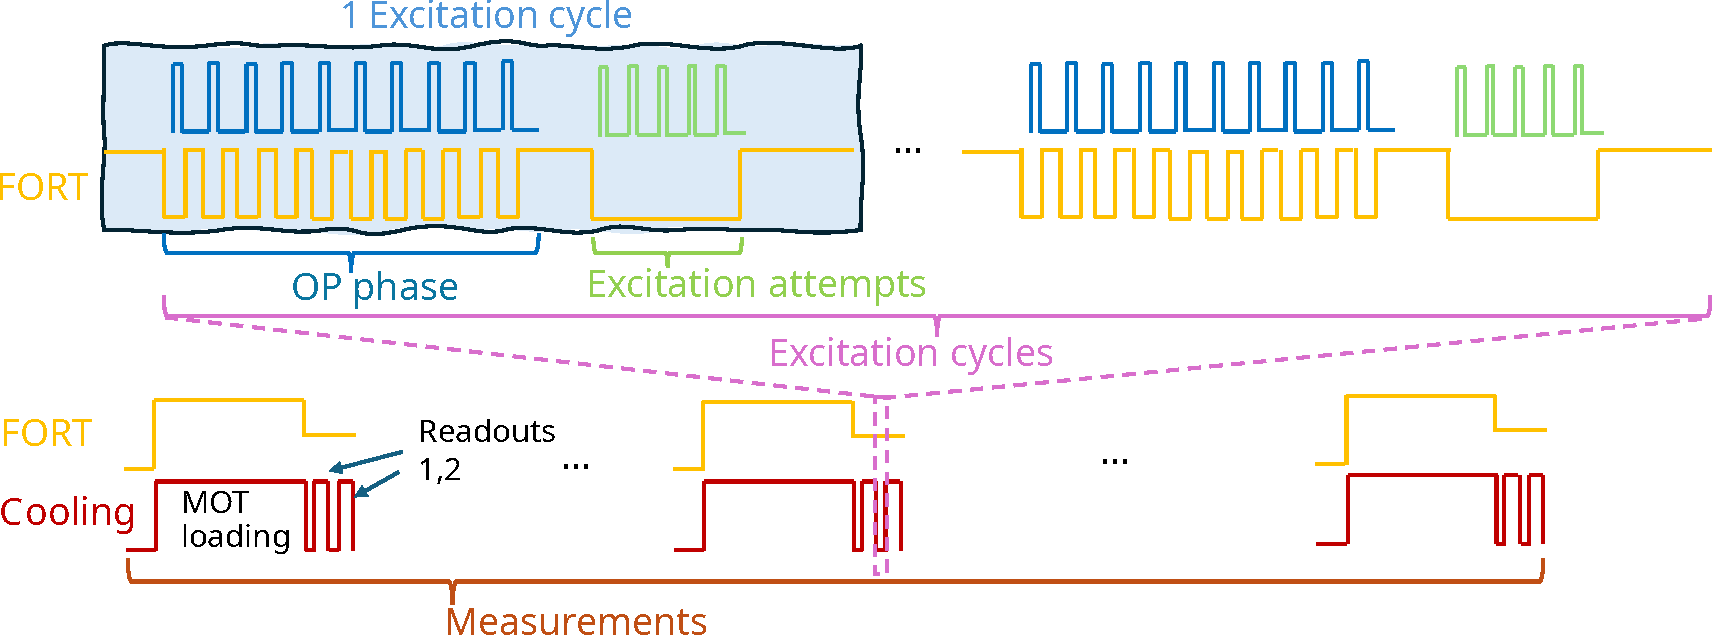
\includegraphics[width=\textwidth]{Images/single_photon_experiment_sequence.pdf}
    \caption{The experiment sequence loop for generating single photons, involving multiple sequences of chopped optical pumping (blue) and excitation attempts (green) per atom loaded. The nomenclature shown is used for consistency with what is used in the lab.}
    \label{fig:single_photon_sequence}
\end{figure}

The experiment sequence loop for generating single photons is shown in Fig. \ref{fig:single_photon_sequence}. For each atom loading attempt, multiple excitation cycles, defined as optically pumping the atom into $\ket{F=1,m_F=0}$ followed by at least one excitation pulse, are done in series several times. The exact number is chosen based on how likely the atom is to survive at the end of several cycles. For example, without adding in a recooling cycle, we observe that the atom survival probability after 10 excitation attempts is around 60$\%$ (Fig. \ref{fig:sequence_survival_probability}). Note that multiple excitation pulses in series may be used without worry of more than one photon collected per series of excitation pulses, as the atom either decays into the $F=1$ stretched states which are dark to the excitation light, or it decays back to the inital state, the emission of which is $\pi$-polarized so we do not collect it (if the bias field is tuned correctly to be along the axis of the collection optics). Using several excitation pulses this way allows us to fight the per-pulse probability of $2/3$ to get $\sigma$-polarized emission and get probability approaching 1 after several attempts. Since the optical pumping takes an order of magnitude longer than the excitation pulse, even in the best case, it is advantageous to have multiple excitation pulses in series. 

\begin{figure}[!h]
    \centering
    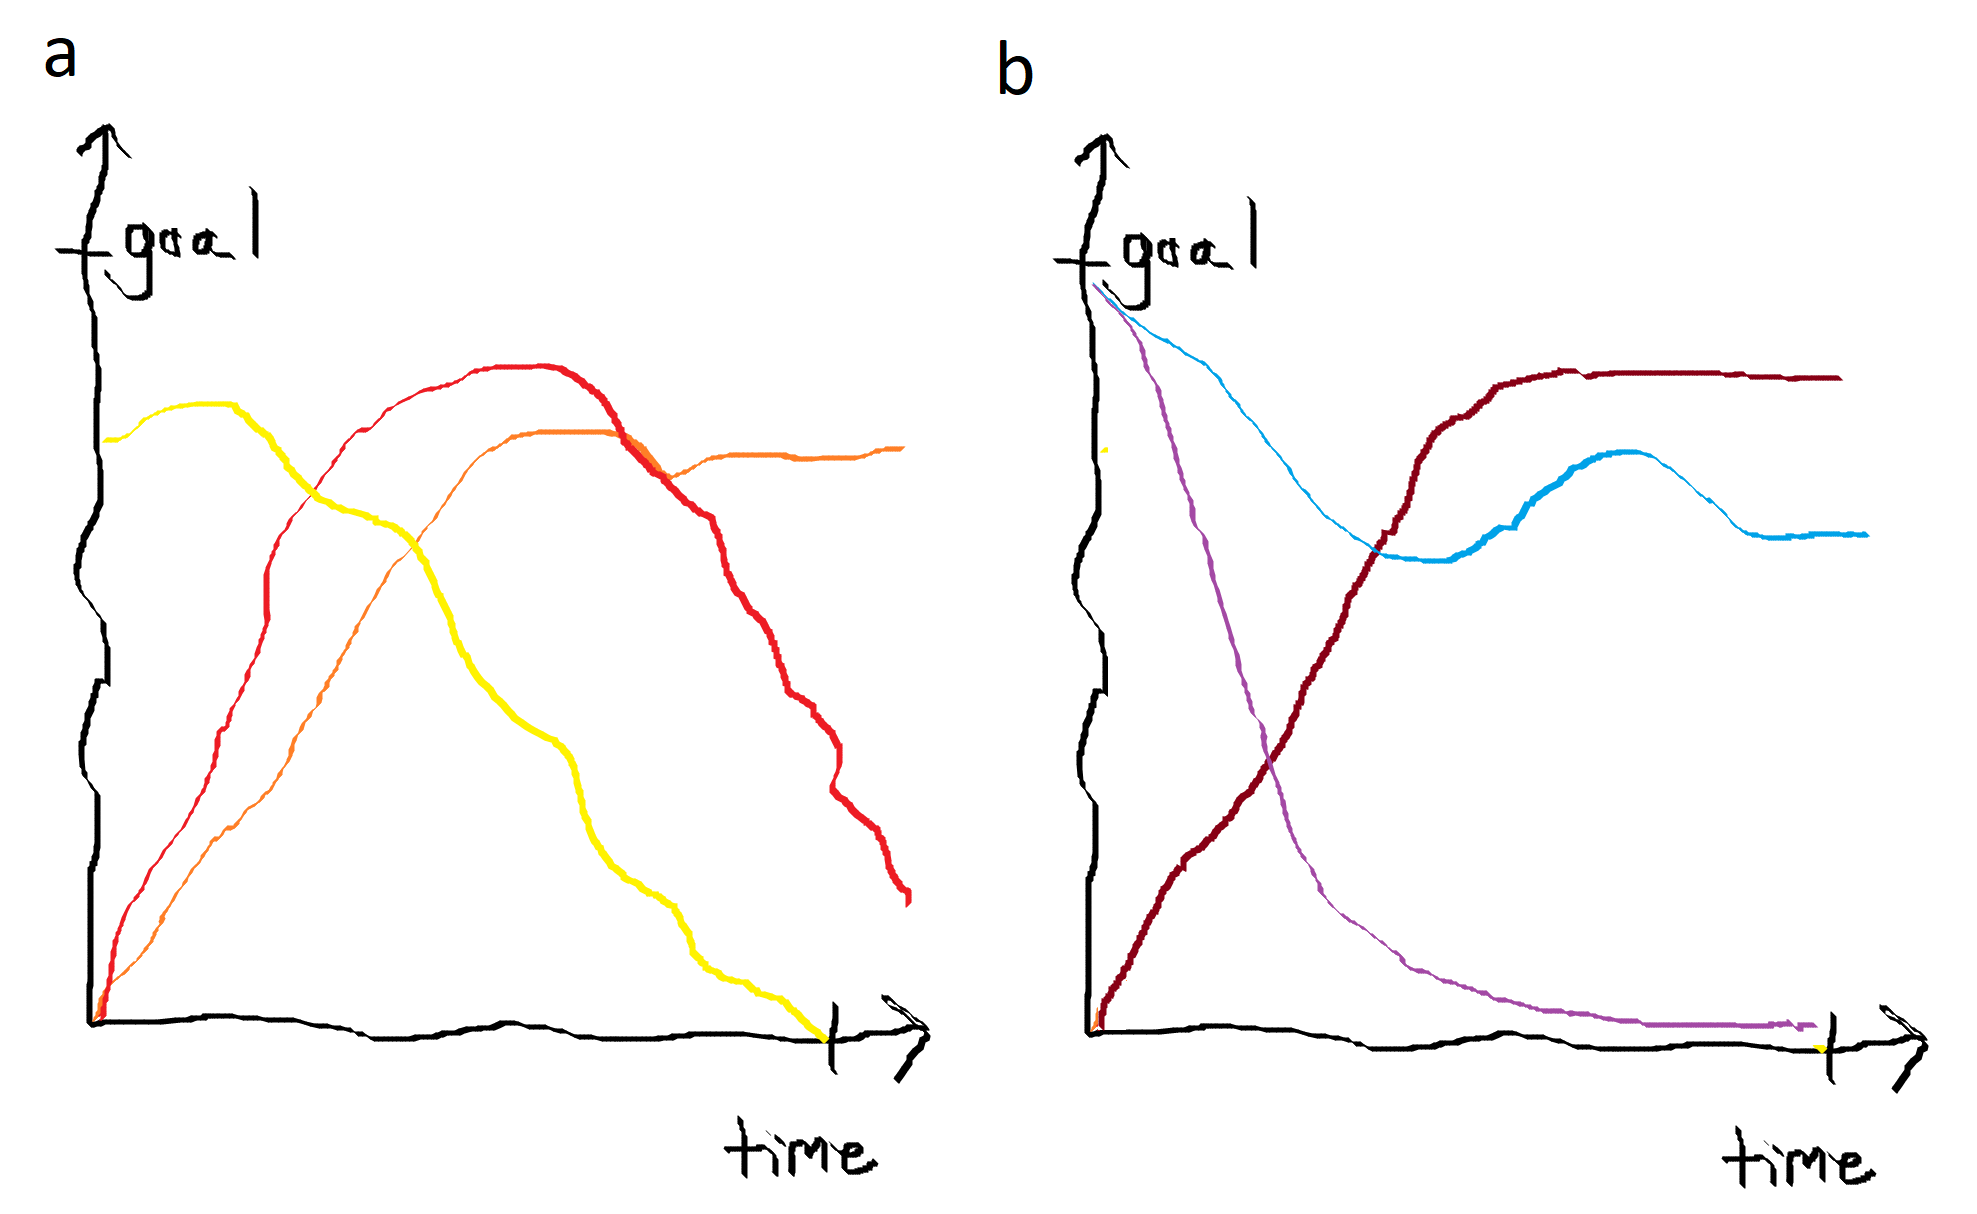
\includegraphics[width=\textwidth]{Images/fig_coming_soon.png}
    \caption{The probability an atom is retained following some number of excitation cycles with no recooling stage.}
    \label{fig:sequence_survival_probability}
\end{figure}




As the lifetime of the $5P_{3/2}$ states is only 27 ns, we would like to excite the atom in less time than this to mitigate decay during the excitation, as this can lead to an effective jitter in the arrival time of photons due to decay during the excitation. Short pulses are broader in frequency and can potentially lead to unwanted excitation. The nearest state that could be excited off-resonantly is $\ket{5P_{3/2},F=2,m_F=0}$, which is nearly 230 MHz away (note that the $\ket{5S_{1/2},F=1,m_F=0} \leftrightarrow \ket{5P_{3/2},F=1,m_F=0}$ transition is electric dipole forbidden because $F$ and $m_F$ do not change). Thus for a pulse of width $\sim$10 ns, we can safely neglect off-resonant driving.

The excitation light, pulsed by an AOM, can be approximated by a Gaussian pulse in order to estimate how much power we need at the atoms for a given pulse width. The requirement to complete full population transfer with a time-varying Rabi frequency is 
\begin{equation}
\int_{t_1}^{t_2} \Omega(t') dt' =\pi
\end{equation}
For $\Omega(t)=\Omega_0 \exp({-\frac{t^2}{2\tau^2}})$, taking $t_1=-\infty$, and $t_2=\infty$ (most of the pule area is contained in a much shorter duration but this allows for a clean analytical result) and we have
\begin{equation} \label{eq:pi}
\begin{split}
\pi & = \Omega_0 \tau \sqrt{2 \pi} \\
 & = \Omega_0 \sqrt{2 \pi} \frac{t_{\textrm{FWHM}}}{2\sqrt{2\ln(2)}} \\
 & = \Omega_0 \sqrt{\pi} \frac{t_{\textrm{FWHM}}}{2\sqrt{\ln(2)}} \\
\end{split}
\end{equation}
which gives
\begin{equation}
    \Omega_0=\frac{2\sqrt{\pi \ln(2)}}{t_{\textrm{FWHM}}}
\end{equation}

% $\pi = \Omega_0 \tau \sqrt{2 \pi}$
% $= \Omega_0 \sqrt{2 \pi} \frac{t_{\textrm{FWHM}}}{2\sqrt{2\ln(2)}}$
% $= \Omega_0 \sqrt{\pi} \frac{t_{\textrm{FWHM}}}{2\sqrt{\ln(2)}}$
% $\Omega_0=\frac{2\sqrt{\pi \ln(2)}}{t_{\textrm{FWHM}}}$

Now we can calculate the power required to have $\Omega_0$ given a beam with a Gaussian spatial intensity pattern with $1/e^2$ waist $w_0$. 
\begin{equation}
    \Omega_0=\frac{dE}{\hbar}
\end{equation}
\begin{equation}
    I_0=\frac{2P_0}{\pi w_0^2}=\frac{1}{2}c \epsilon_0|E|^2
\end{equation}
\begin{equation}
    \Omega_0 =\frac{d}{\hbar}\sqrt{\frac{2I_0}
{c\epsilon_0}}=\frac{d}{\hbar}\sqrt{\frac{4P_0}{c\epsilon_0 \pi w_0^2}}
\end{equation}

Solving for $P_0$ gives
\begin{equation}\label{eq:p0}
\begin{split}
P_0 & = \frac{\hbar^2}{4d^2}\Omega_0^2\pi w_0^2 c \epsilon_0 \\
 & = \frac{\hbar^2}{4d^2} \pi w_0^2 c \epsilon_0 \left(\frac{2\sqrt{\pi \ln(2)}}{t_{\textrm{FWHM}}}\right)^2 \\
 & = \frac{\hbar^2}{d^2} \pi^2 w_0^2 c \epsilon_0\frac{\ln(2)}{t_{\textrm{FWHM}}^2} \\
\end{split}
\end{equation}
resulting in the peak Rabi frequency
\begin{equation}\label{eq:omega0}
    \Omega_0=\frac{2\sqrt{\pi \ln(2)}}{t_{\textrm{FWHM}}}.
\end{equation}
It can be shown with dimensional analysis that the units above (Eq. \ref{eq:omega0}) are in fact power\footnote{Left as an exercise for the younger grad students.}.

The electric dipole matrix element for a transition $F,m_F$ to $F',m_F'$ on the $^{87}\textrm {Rb}$  $D_2$ line is given by
\begin{equation}d=4.227 e a_0 (-1)^{F'+J+1+I} \sqrt{(2 F'+1)(2 J+1)}\left\{\begin{array}{ccc}
J & J' & 1 \\
F' & F & I
\end{array}\right\}C_{F,m_F;1,-q}^{F',m_F'}
\end{equation}
where $\left\{ \begin{array}{c} \dots \\ \dots \end{array} \right\}$ is a Wigner $6j$ symbol, with $J=1/2$, $J'=3/2$, and $I=3/2$. The numerical prefactor times $e a_0$ is the fine structure reduced matrix element. Note that I use the convention $q = m_F' - m_F$, which opposite of what is used by others, e.g. Steck.
For $F=1, m_F=0$,  $F'=0, m_F'=0$, and linear polarization ($q=0$), we get
$|d|=5.636*10^{-30} ~\textrm{C}\cdot\textrm{m}$.
Now, we can evaluate what peak power we need to drive the $\pi$ rotation. The beam waist from either GRIN lens is about 300 $\mu \textrm{m}$. We can solve for the power with the relations above to get
\begin{equation}
    P_0 = c \epsilon_0 \pi^2 w_0^2 \frac{\hbar^2 \ln(2)}{d^2 t_{\textrm{FWHM}}^2}
\end{equation}
Using $t_{\textrm{FWHM}}=20~ \textrm{ns}$, we find $P_0 = 212~\mu \textrm{W}$.

As a sanity check, we can compare with a square pulse, for which the Rabi frequency needed is simply
\begin{equation}
    \Omega = \frac{\pi}{t}
\end{equation}
where $t$ is the pulse length. From the derivation above, we see \begin{equation}
    \frac{\Omega_{\textrm{square}}}{\Omega_{\textrm{Gaussian}}}=\frac{1}{2}\sqrt{\frac{\pi}{\ln(2)}} \approx 1.06
\end{equation}
The Rabi frequency scales as the square root of the power, so we have
\begin{equation}
\frac{P_{\textrm{square}}}{P_{\textrm{Gaussian}}} \approx 1.12
\end{equation}
Evidently, one needs about $10\%$ more power to excite the atom with a Gaussian pulse of the same nominal temporal length.

\section{Next steps}


